\subsection{Person}

Finally, one of the main error sources of HPE is the person. The person can cause difficulties in the HPE process by moving, wearing specific clothes, or having a different body posture. Body posture is of special importance for SilverFit since SilverFit specialises in games for rehabilitation and elderly people. Elderly people have different body postures than the average person, which can cause difficulties in the HPE process.

\subsubsection{Clothes}

As mentioned earlier, most RGB-D cameras use infrared light to determine the depth of the scene. This means that the clothes of the user can cause more or less absorption of light and therefore influence the detected depth. This can cause the joints to be detected in the wrong position or not at all. This is especially the case for dark clothes, as they absorb more light than light clothes.

Furthermore, bulky clothes or skirts and dresses may influence the pose, since the exact position of the legs is not visible.

\subsubsection{Training Equipment}

To make exercises more challenging some physiotherapists use additional training equipment. This could be weights that are held in the hand or weights that are attached to the ankles. These weights change the outline of the body and therefore influence the pose estimation. 

\subsubsection{Exercises}
\label{sec:exercises}

Finally, the most important factor is the exercise that is carried out. In this section, both exercises that are easy to detect as well as some exercises that are difficult to detect are proposed.

These exercises might not be the most realistic, but they represent common issues with pose estimation in a reproducible manner. Furthermore, these exercises are not too difficult to perform, which makes them suitable for testing the pose estimators. The difficulty rating of the exercise might not reflect the difficulty of the exercise for the user, but it does reflect the difficulty of the exercise for the pose estimator.

The exercises are numbered according to the difficulty. An example of the naming of the exercises can be seen here:

\[
    \underbrace{E}_\text{Exercise}-\overbrace{2}^\text{Difficulty}.\underbrace{02}_\text{Exercise Id}
\]

The different difficulties are numbered as follows:

\begin{enumerate}
    \addtocounter{enumi}{-1}
    \item Trivial
    \item Easy
    \item Medium
    \item Hard
\end{enumerate}

\paragraph{Trivial Exercises}

Trivial exercises are exercises that are easy to detect and are therefore good for testing the pose estimators. The exercises do not involve any movement, which makes detecting the joints easier. The two trivial exercises can be seen in table \ref{tab:trivial_exercises}. Example images of the exercises can be seen in figure \ref{fig:trivial_exercises}.

\begin{table}[ht]
  \caption[Trivial Exercises]{The two Trivial Exercises, E-0.00 and E-0.01.}
  \label{tab:trivial_exercises}
  \begin{tabular}{p{0.1\linewidth}p{0.3\linewidth}p{0.55\linewidth}}
  \hline
  Exercise & Short Description         & challenge   \\ \hline
  E-0.00   & Arms hanging to the side  & This exercise is very easy since no part of the body is occluded by any other part. Additionally, the joints are not moving. \\
  E-0.01   & Arms extended to the side & The arms are no longer in a natural position but still not occluded and no joint is moving \\ \hline
  \end{tabular}
\end{table} 

\begin{figure}[ht]
  \centering
  \begin{subfigure}[b]{0.32\linewidth}
      \centering
      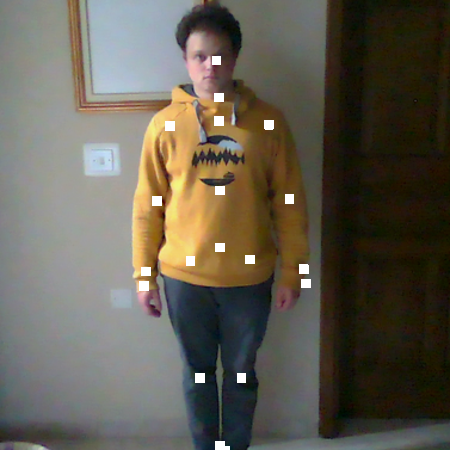
\includegraphics[width=\textwidth]{figures/Data/samples/trivial/E-0.00_10.png}
      \caption[]{E-0.00}
      \label{fig:trivial_0}
  \end{subfigure}
  \hfill
  \begin{subfigure}[b]{0.32\linewidth}
      \centering
      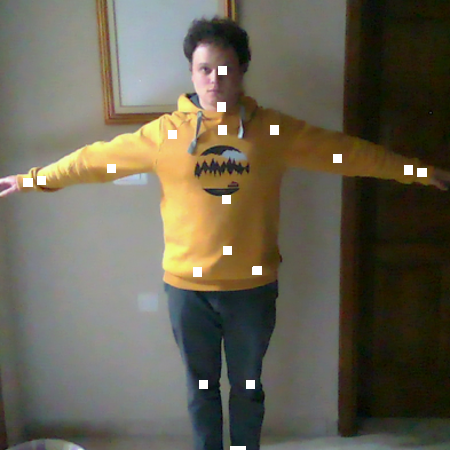
\includegraphics[width=\textwidth]{figures/Data/samples/trivial/E-0.01_38.png}
      \caption[]{E-0.01}
      \label{fig:trivial_1}
  \end{subfigure}
  \caption[Trivial Exercises]{The two trivial exercises. (\ref{fig:trivial_0}) Arms hanging to the side. (\ref{fig:trivial_1}) Arms extended to the side.}
  \label{fig:trivial_exercises}
\end{figure}  

\paragraph{Easy Exercises}

Easy exercises are essential for creating a good baseline of how the pose estimators should work. The exercises include no self-occlusion and are recorded in a standing position, which is generally the easiest position to detect. The easy exercises can be seen in table \ref{tab:easy_exercises}. Example images of the exercises can be seen in figure \ref{fig:easy_exercises}.

\begin{table}[ht]
  \caption[Easy Exercises]{The Easy exercises, E-1.00 through E-1.03. The easy exercises include both standing and sitting exercises.}
  \label{tab:easy_exercises}
  \begin{tabular}{p{0.1\linewidth}p{0.3\linewidth}p{0.55\linewidth}}
  \hline
  Exercise & Short Description             & Challenge \\ \hline
  E-1.00   & Raising the arms to the side  & Now the arms are no longer stationary. Still, there is no Occlusion. \\
  E-1.01   & Raising the arms to the front & The arms might occlude themselves and part of the body.  \\
  E-1.02   & Raise the knees to the chest  & The legs now occlude parts of the hip.  \\
  E-1.03   & Sit in a chair motionless     & Sitting positions are more challenging to detect than standing positions since there is now a chair in the background and the body occludes itself.\\ \hline
  \end{tabular}
  \end{table}

  \begin{figure}[ht]
    \centering
    \begin{subfigure}[b]{0.32\linewidth}
        \centering
        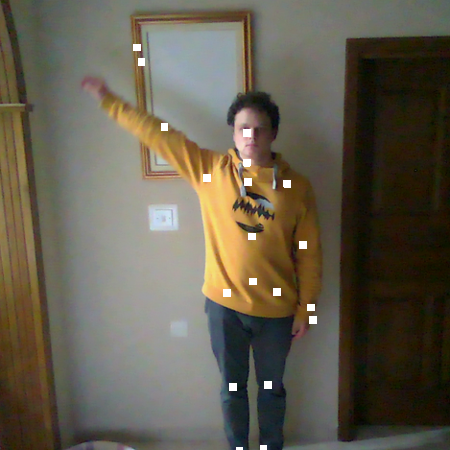
\includegraphics[width=\textwidth]{figures/Data/samples/easy/E-1.00_126.png}
        \caption[]{E-1.00}
        \label{fig:easy_0_0}
    \end{subfigure}
    \hfill
    \begin{subfigure}[b]{0.32\linewidth}
        \centering
        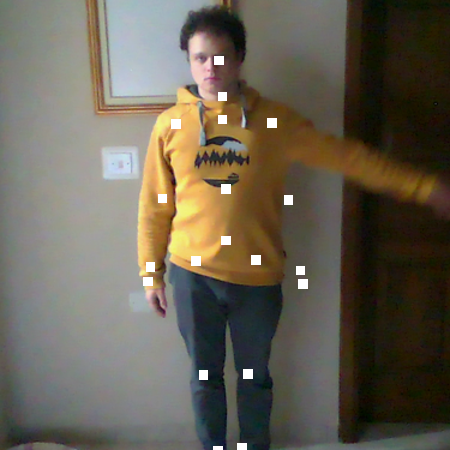
\includegraphics[width=\textwidth]{figures/Data/samples/easy/E-1.00_137.png}
        \caption[]{E-1.00}
        \label{fig:easy_0_1}
    \end{subfigure}
    \hfill
    \begin{subfigure}[b]{0.32\linewidth}
        \centering
        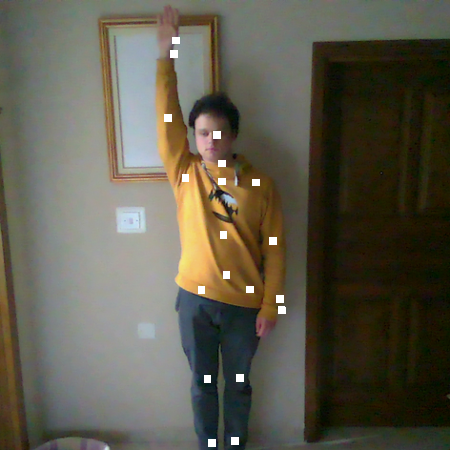
\includegraphics[width=\textwidth]{figures/Data/samples/easy/E-1.01_188.png}
        \caption[]{E-1.01}
        \label{fig:easy_1_0}
    \end{subfigure}
    \hfill
    \begin{subfigure}[b]{0.32\linewidth}
        \centering
        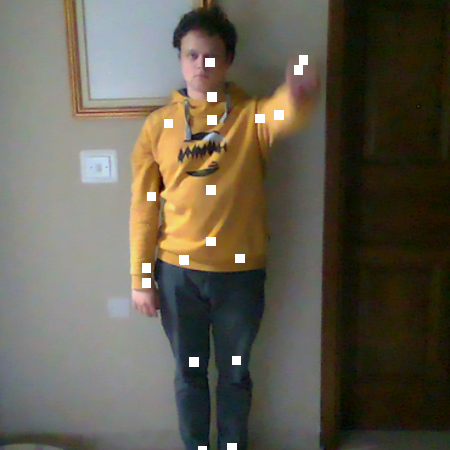
\includegraphics[width=\textwidth]{figures/Data/samples/easy/E-1.01_197.png}
        \caption[]{E-1.01}
        \label{fig:easy_1_1}
    \end{subfigure}
    \hfill
    \begin{subfigure}[b]{0.32\linewidth}
        \centering
        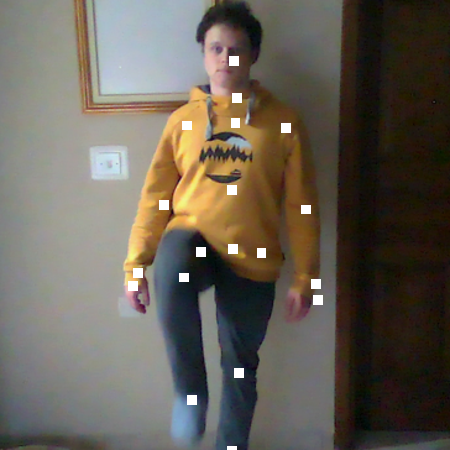
\includegraphics[width=\textwidth]{figures/Data/samples/easy/E-1.02_230.png}
        \caption[]{E-1.02}
        \label{fig:easy_2_0}
    \end{subfigure}
    \hfill
    \begin{subfigure}[b]{0.32\linewidth}
        \centering
        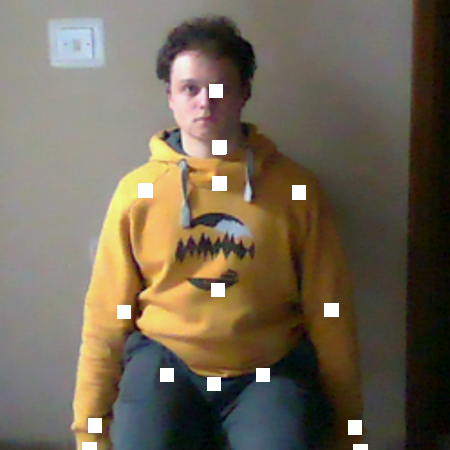
\includegraphics[width=\textwidth]{figures/Data/samples/easy/E-1.03_301.png}
        \caption[]{E-1.03}
        \label{fig:easy_3_0}
    \end{subfigure}
    \caption[Easy Exercises]{The four easy exercises. (\ref{fig:easy_0_0}, \ref{fig:easy_0_1}) Raising the arms to the side. (\ref{fig:easy_1_0}, \ref{fig:easy_1_1}) Raising the arms to the front. (\ref{fig:easy_2_0}) Raising the knee to the chest. (\ref{fig:easy_3_0}) Sitting in a chair motionless.}
    \label{fig:easy_exercises}
  \end{figure}  

\paragraph{Medium Exercises}

Exercises which are performed in a seated position are harder to detect since parts of the body are occluded. Medium exercises focus on exercises, which are performed in a seated position. The medium exercises can be seen in table \ref{tab:medium_exercises}. Example images of the exercises can be seen in figure \ref{fig:medium_exercises}.

\begin{table}[ht]
  \caption[Medium Exercises]{The Medium exercises, E-2.00 through E-2.03. The medium exercises are all in a sitting position.}
  \label{tab:medium_exercises}
  \begin{tabular}{p{0.1\linewidth}p{0.3\linewidth}p{0.55\linewidth}}
  \hline
  Exercise & Short Description                                     & Challenge \\ \hline
  E-2.00   & Raising the arms to the side while sitting            & Now the arms are no longer stationary. With added difficulty since the user is now sitting.         \\
  E-2.01   & Raising the arms to the front while sitting           & The arms might occlude themselves and part of the body. Additionally, the person is now sitting down\\
  E-2.02   & Crossing the arms in front of the chest while sitting & The arms now occlude large parts of the upper body.                                                                                            \\
  E-2.03   & Raising the knee to the chest while sitting           & More parts of the upper body are occluded and not seen by the camera.                              \\ \hline
  \end{tabular}
  \end{table}

  \begin{figure}[ht]
    \centering
    \begin{subfigure}[b]{0.32\linewidth}
        \centering
        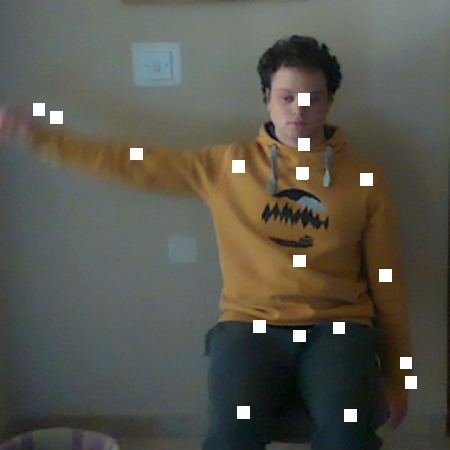
\includegraphics[width=\textwidth]{figures/Data/samples/medium/E-2.00_365.png}
        \caption[]{E-2.00}
        \label{fig:medium_0_0}
    \end{subfigure}
    \hfill
    \begin{subfigure}[b]{0.32\linewidth}
        \centering
        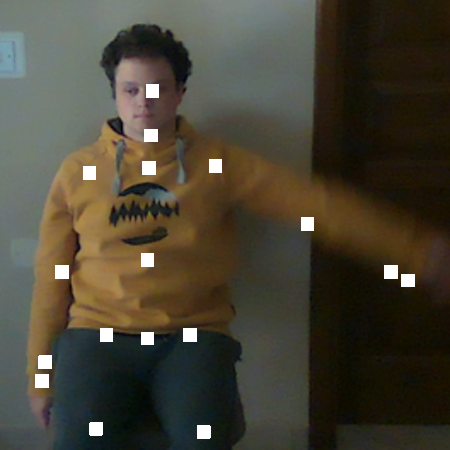
\includegraphics[width=\textwidth]{figures/Data/samples/medium/E-2.00_385.png}
        \caption[]{E-2.00}
        \label{fig:medium_0_1}
    \end{subfigure}
    \hfill
    \begin{subfigure}[b]{0.32\linewidth}
        \centering
        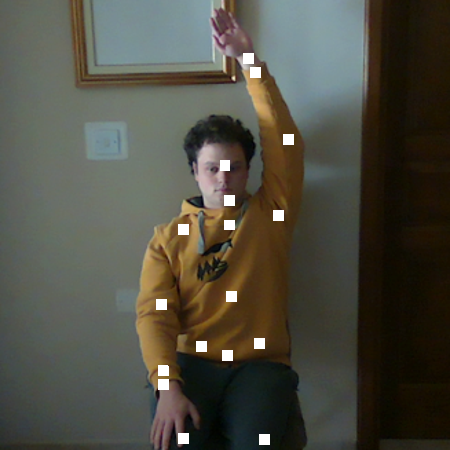
\includegraphics[width=\textwidth]{figures/Data/samples/medium/E-2.01_440.png}
        \caption[]{E-2.01}
        \label{fig:medium_1_0}
    \end{subfigure}
    \hfill
    \begin{subfigure}[b]{0.32\linewidth}
        \centering
        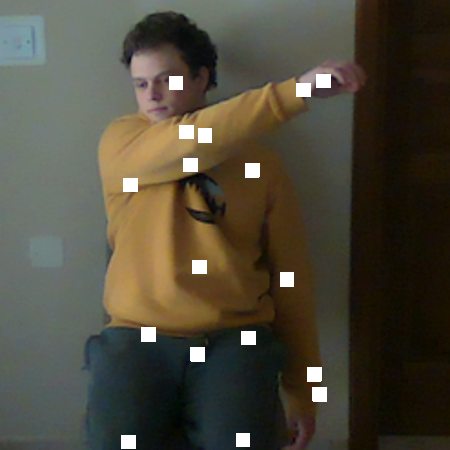
\includegraphics[width=\textwidth]{figures/Data/samples/medium/E-2.02_487.png}
        \caption[]{E-2.02}
        \label{fig:medium_2_0}
    \end{subfigure}
    \hfill
    \begin{subfigure}[b]{0.32\linewidth}
        \centering
        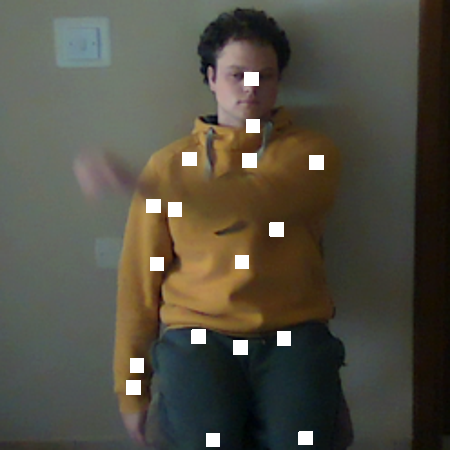
\includegraphics[width=\textwidth]{figures/Data/samples/medium/E-2.02_500.png}
        \caption[]{E-2.02}
        \label{fig:medium_2_1}
    \end{subfigure}
    \hfill
    \begin{subfigure}[b]{0.32\linewidth}
        \centering
        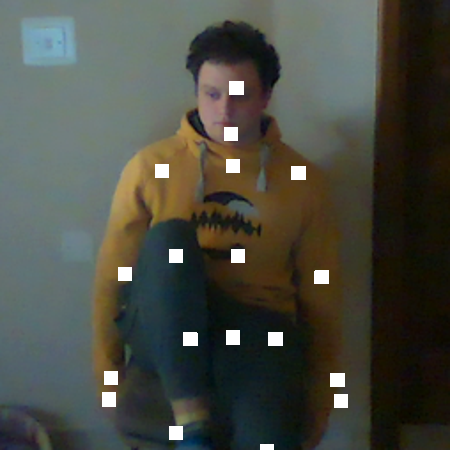
\includegraphics[width=\textwidth]{figures/Data/samples/medium/E-2.03_590.png}
        \caption[]{E-2.03}
        \label{fig:medium_3_0}
    \end{subfigure}
    \caption[Medium Exercises]{The four medium exercises. (\ref{fig:medium_0_0}, \ref{fig:medium_0_1}) Raising the arms to the side while sitting. (\ref{fig:medium_1_0}) Raising the arms to the front while sitting. (\ref{fig:medium_2_0}, \ref{fig:medium_2_1}) Crossing the arms in front of the chest while sitting. (\ref{fig:medium_3_0}) Raising the knee up to the chest while sitting.}
    \label{fig:medium_exercises}
  \end{figure}  

\paragraph{Difficult Exercises}

Difficult exercises are exercises that are performed in a standing position and involve leg movement. Leg joints are harder to detect than arm joints and therefore pose a greater challenge for pose estimators. These exercises will be in a seating position and with a difficult posture, such as leaning forward. The difference in posture aims at creating a realistic representation of real-world exercises.

Tölgyessy et al. found that facing away from the camera decreases the accuracy of HPE due to self-occlusion. \cite{HPEIsHard} Therefore, some of the exercises will be performed facing away from the camera. The difficult exercises can be seen in table \ref{tab:difficult_exercises}. Example images of the exercises can be seen in figure \ref{fig:difficult_exercises}.

\begin{table}[ht]
  \caption[Difficult Exercises]{The Difficult exercises, E-3.00 through E-3.02. The difficult exercises are all in a standing position.}
  \label{tab:difficult_exercises}
  \begin{tabular}{p{0.1\linewidth}p{0.3\linewidth}p{0.55\linewidth}}
  \hline
  Exercise & Short Description                                                              & Challenge \\ \hline
  E-3.00   & Bowing toward the camera                                                       & The head is often used as an anchor point for the skeleton as it is quite stable. When bowing forward the head is no longer easily detectable. \\
  E-3.01   & Raising the knee leaning forward                                               & Leaning forward increases the difficulty since the position is not natural \\
  E-2.02   & Raising the knee leaning forward while sitting and facing away from the camera & Facing away from the camera makes it more difficult to detect the pose and induces more occlusion.  \\ \hline
  \end{tabular}
\end{table}

\begin{figure}[ht]
  \centering
  \begin{subfigure}[b]{0.32\linewidth}
      \centering
      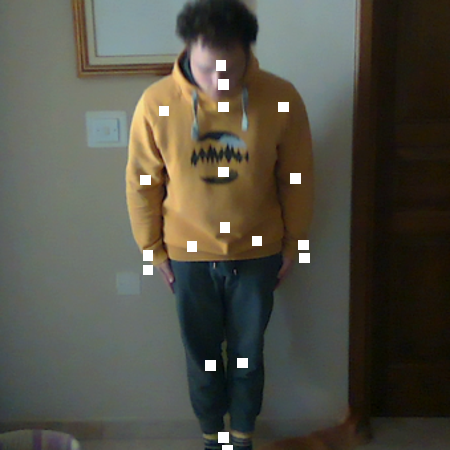
\includegraphics[width=\textwidth]{figures/Data/samples/hard/E-3.00_530.png}
      \caption[]{E-3.00}
      \label{fig:hard_0_0}
  \end{subfigure}
  \hfill
  \begin{subfigure}[b]{0.32\linewidth}
      \centering
      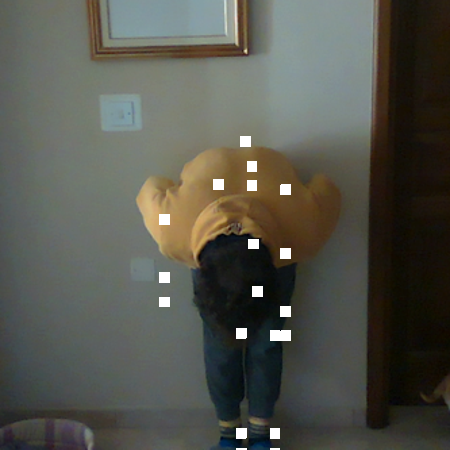
\includegraphics[width=\textwidth]{figures/Data/samples/hard/E-3.00_535.png}
      \caption[]{E-3.00}
      \label{fig:hard_0_1}
  \end{subfigure}
  \hfill
  \begin{subfigure}[b]{0.32\linewidth}
      \centering
      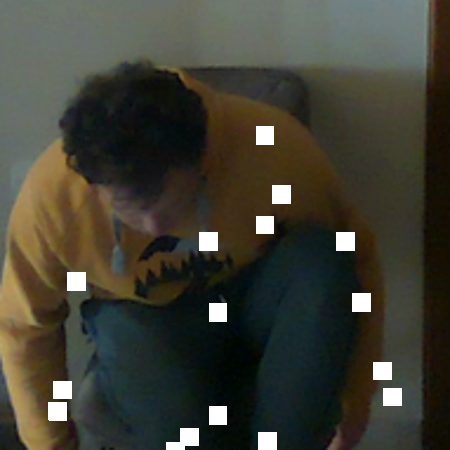
\includegraphics[width=\textwidth]{figures/Data/samples/hard/E-3.01_635.png}
      \caption[]{E-3.01}
      \label{fig:hard_1_0}
  \end{subfigure}
  \hfill
  \begin{subfigure}[b]{0.32\linewidth}
      \centering
      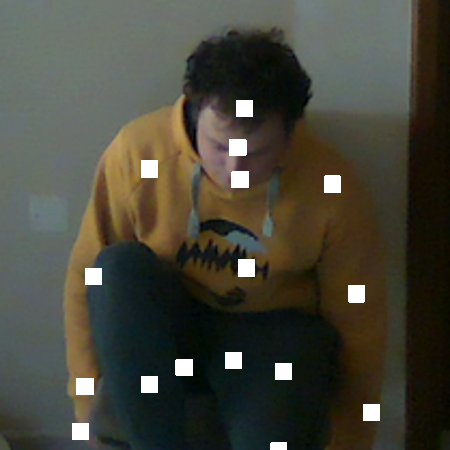
\includegraphics[width=\textwidth]{figures/Data/samples/hard/E-3.01_685.png}
      \caption[]{E-3.01}
      \label{fig:hard_1_1}
  \end{subfigure}
  \hfill
  \begin{subfigure}[b]{0.32\linewidth}
      \centering
      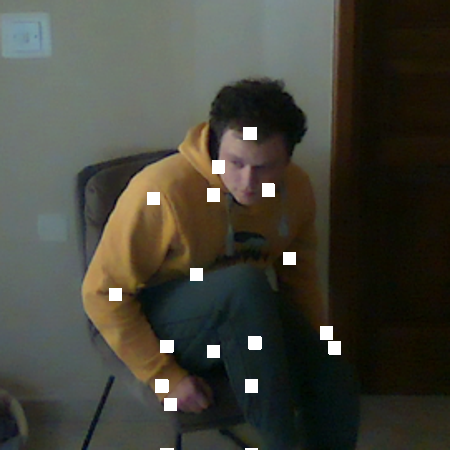
\includegraphics[width=\textwidth]{figures/Data/samples/hard/E-3.02_695.png}
      \caption[]{E-3.02}
      \label{fig:hard_2_0}
  \end{subfigure}
  \hfill
  \begin{subfigure}[b]{0.32\linewidth}
      \centering
      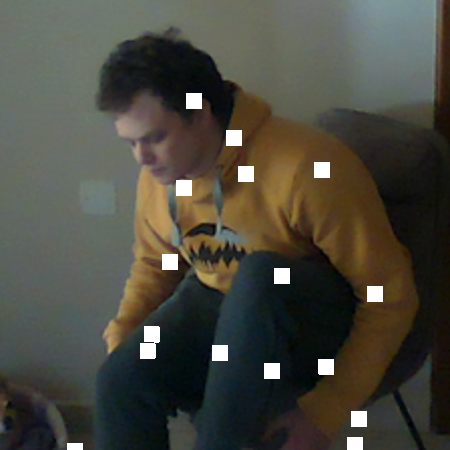
\includegraphics[width=\textwidth]{figures/Data/samples/hard/E-3.02_725.png}
      \caption[]{E-3.02}
      \label{fig:hard_2_1}
  \end{subfigure}
  \caption[Difficult Exercises]{The three difficult exercises. (\ref{fig:hard_0_0} \ref{fig:hard_0_1}) Bowing toward the camera. (\ref{fig:hard_1_0}, \ref{fig:hard_1_1}) Raising the knee leaning forward. (\ref{fig:hard_2_0}, \ref{fig:hard_2_1}) Raising the knee leaning forward while sitting and facing away from the camera. Some of the exercises contain errors in the sample.}
  \label{fig:difficult_exercises}
\end{figure}
